A ferramenta StArt -- \textit{State of the Art through Systematic Review} \cite{fabbri2013} -- foi desenvolvida para fornecer suporte computacional para o maior número possível de atividades de uma Revisão Sistemática, desde o preenchimento do protocolo na fase de planejamento, passando pelas atividades de seleção inicial e extração de dados na fase de execução, até a fase de sumarização dos dados.

\begin{enumerate}

    \item \textbf{Fase de Planejamento}
    
    Em relação ao planejamento, o protocolo trazido pela ferramenta possui os mesmos campos propostos por \citet{Kitchenham2011} para auxiliar os pesquisadores na condução da revisão sistemática e também na repetitividade do processo. Permite o registro de informações tais como objetivo, questões de pesquisa, métodos utilizados para seleção, palavras-chave utilizadas nas strings de busca, critérios de inclusão e exclusão, máquinas de busca utilizadas, formulário de extração, descrição de critérios de qualidade e de como a sumarização será feita. A \textit{Figura \ref{Start01}} mostra alguns campos do protocolo existente na ferramenta.
    
    \begin{figure}[!htb]
	\centering
	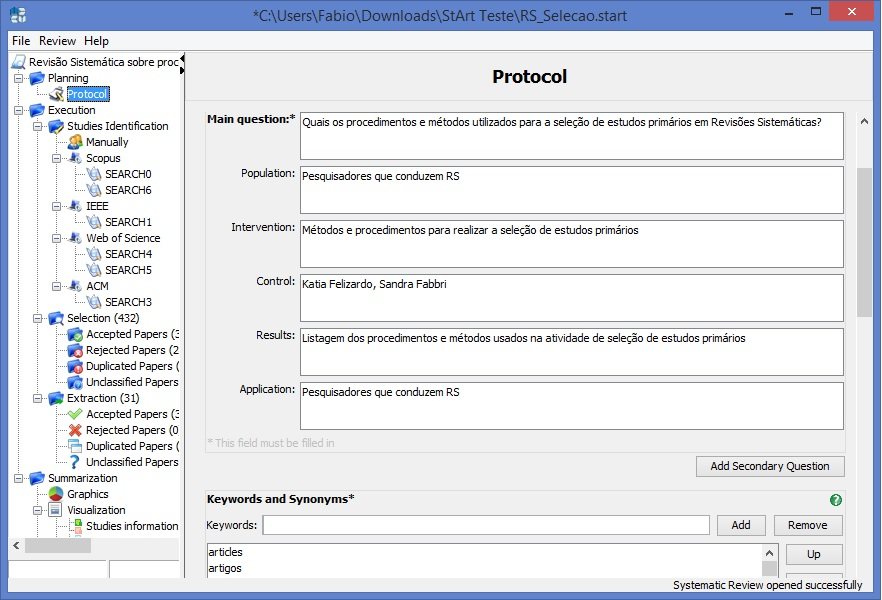
\includegraphics[scale=0.65]{Capitulo-Apendices/figura/Start01.jpg}
	\caption{Formulário de protocolo da ferramenta StArt}
	\label{Start01}
    \end{figure}
    
    \item \textbf{Fase de Execução}
    
    Em relação à execução, a ferramenta permite que os estudos primários recuperados das máquinas de busca sejam carregados por meio de arquivos exportados de várias máquinas de busca no formato BibTex, RIS, MedLine ou Cochrane. Artigos duplicados são detectados automaticamente pela ferramenta por meio de técnicas de mineração de texto.
    
    Além disso, a StArt traz um importante recurso para auxiliar os pesquisadores na seleção inicial de estudos primários: o score. Esse recurso considera a frequência com que as \textit{keywords} definidas no protocolo aparecem no título, \textit{abstract} e palavras-chave dos estudos primários recuperados, fazendo um ranqueamento de estudos. Quanto maior o score de um estudo, maior é a sua chance de ser relevante ao tema de pesquisa. A \textit{Figura \ref{Start02}} mostra um exemplo de tela da StArt no qual os estudos são classificados por score.
    
    \begin{figure}[!htb]
	\centering
	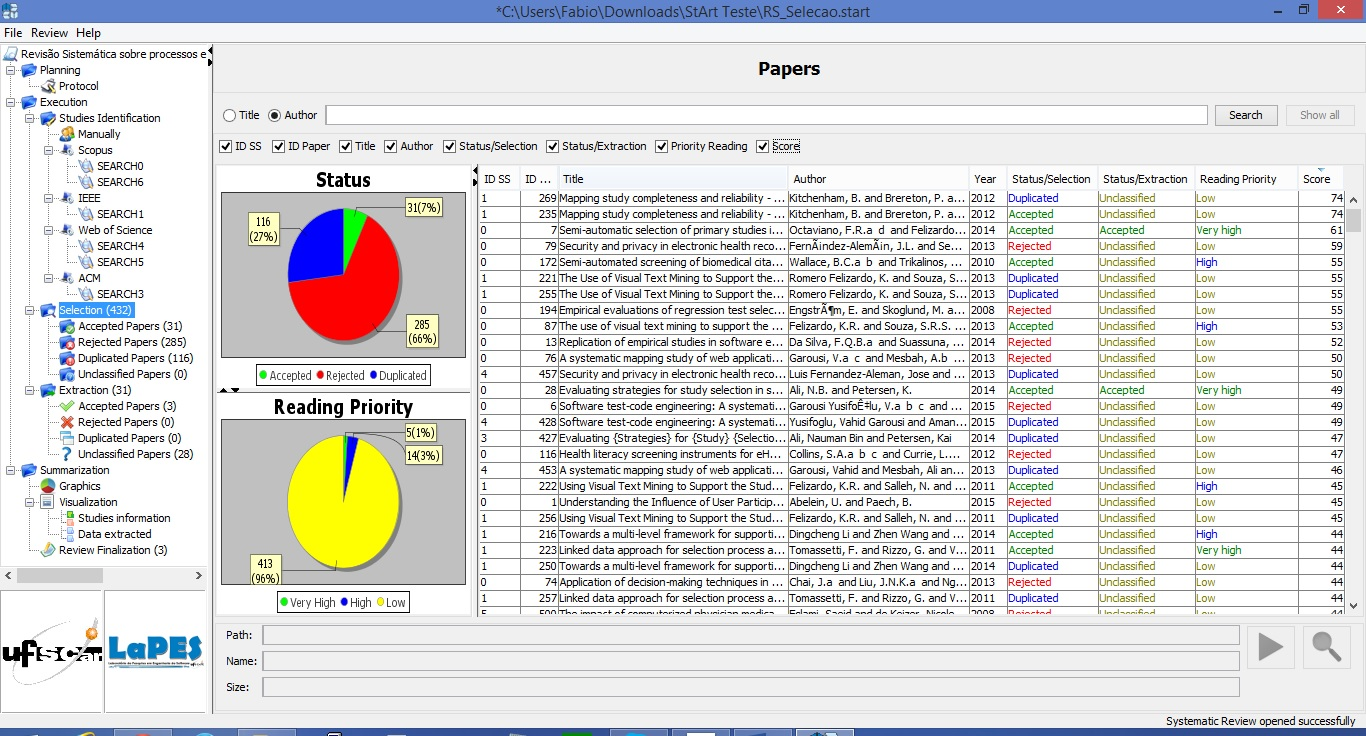
\includegraphics[scale=0.45]{Capitulo-Apendices/figura/Start02.jpg}
	\caption{Estudos classificados por score na atividade de seleção inicial}
	\label{Start02}
    \end{figure}
    
    Um recurso adicional que foi implementado e está em fase de aprimoramento é o número de citações entre os estudos primários (cross-citation) carregados na ferramenta. 
    
    Outro recurso existente que pode auxiliar o pesquisador na seleção é o percentual de similaridade de estudos, em que, por meio de mineração de texto, a ferramenta apresenta estudos similares em conteúdo em relação a um estudo selecionado pelo pesquisador. Assim, ao detectar um estudo relevante, é possível navegar por outros estudos com conteúdo similares, que supostamente tendem a ser relevantes também.

    Na etapa de extração, a ferramenta apresenta os campos do formulário de extração definido no protocolo para que as mesmas informações sejam extraídas de todos os estudos.
    
    \item \textbf{Fase de Sumarização dos Dados}
    
    Em relação à sumarização, a StArt apresenta funcionalidades para facilitar a sumarização dos dados, tais como o uso de recursos de visualização e a geração de relatórios no formato Excel de acordo com as necessidades do pesquisador. É possível gerar visualizações nos formatos de grafo, árvore e grafo-radial, e por diversos campos, tais como ano de publicação, autores, locais de eventos, campos do formulário de extração, entre outros.
    
\end{enumerate}